\documentclass{article}
\usepackage[english]{babel}
\usepackage[utf8]{inputenc}
\usepackage{amsmath,amssymb}
\usepackage{parskip}
\usepackage{graphicx}
\graphicspath{ {./MA3210_images/} }

\newcommand\tab[1][1cm]{\hspace*{#1}}

% Margins
\usepackage[top=2.5cm, left=3cm, right=3cm, bottom=4.0cm]{geometry}


\title{MA3210 (Analysis II)}
\author{Jia Cheng}
\date{September 2021}

\begin{document}

\maketitle

\section{Definitions}
\paragraph{Sets}
\begin{align*}
	\mathbb{N}=\mathbb{Z}^+
\end{align*}

\section{Inequalities}
\begin{itemize}
	\item $|a + b| \leq |a| + |b|$
	\item $||a| - |b||\leq |a - b|$
	\item $||a| - |b|| = ||a| - |-b|| \leq |a + b|$
\end{itemize}

\section{Techniques}
\paragraph{Infimum and supremum}
Let $A, B$ be 2 sets of real numbers.\\
Given that $\forall a\in A, \exists b\in B, a\leq b$ we want to show $\sup A \leq \sup B$.\\
There are in general 2 ways to do this.

The direct way is to go from $B$ to $A$. Take arbitrary $a\in A$, then $\exists b\in B, a\leq b\leq \sup B$. Then $\sup B$ is an upper bound of $A$, hence $\sup A\leq \sup B$. We call this going from $B$ to $A$ in the sense that we produce $\sup B$ before producing $\sup A$ in our equations.

The other way goes in the reverse direction. Choose arbitrary $\epsilon>0$, and by definition of supremum, $\exists a\in A$, $\sup A - \epsilon<a\leq \sup A$. Again, there is a $b$ such that $\sup A-\epsilon < a\leq b\leq \sup B$. Hence $\sup A-\epsilon < \sup B$. Since $\epsilon$ is arbitrary, $\sup A\leq \sup B$.

Perhaps a better mnemonic for these 2 ways is that the first goes from the \textit{not pointy} bit of the inequality sign to the \textit{pointy} bit.

\section{Theorem Listing}
\subsection{Inf and sup}
\paragraph{Scalar properties}
Given a bounded set $S\subset \mathbb{R}$
\begin{align*}
\inf(cS)=
\begin{cases}
c\inf(S) \text{ if }c>0\\
c\sup(S) \text{ if }c<0
\end{cases}\\
\sup(cS)=
\begin{cases}
c\sup(S) \text{ if }c>0\\
c\inf(S) \text{ if }c<0
\end{cases}\\
\end{align*}

\paragraph{sup-inf condition}
Let $S$ be a nonempty bounded subset of $\mathbb{R}$ and $K>0$ such that $\forall s,t\in S,|s-t|\leq K$. Then $\sup(S)-\inf(S)\leq K$.

\subsection{Continuity}
\paragraph{Lipschitz property implies uniform continuity}
Lipschitz property: There is a constant $K$, such that for all $x,y$, $|f(x)-f(y)|\leq K|x-y|$.\\
It is then trivial to derive uniform continuity.

\subsection{Differential Calculus}
\paragraph{Caratheodory's Theorem}
Let $f: I\rightarrow \mathbb{R}$, $c\in I$. Then $f'(c)$ exists iff there is a function $\phi: I\rightarrow \mathbb{R}$ such that $\phi$ continuous at $c$ and
\begin{align*}
	\forall x\in I, f(x)-f(c) = \phi(x)(x-c)
\end{align*}
When this is the case, $\phi(c) = f'(c)$.

\paragraph{Inverse Function Lemma}
Let $f:I\rightarrow \mathbb{R}$ be strictly monotone and continuous on $I$. Let $J=f(I)$ such that $f^{-1}:J\rightarrow \mathbb{R}$ inverts $f$ (technically, we need to restrict the codomain of $f$ and $f^{-1}$ to just their range). Suppose $f$ differentiable at $c$ and $f'(c)\neq 0$. Then let $d=f(c)$ and
\begin{align*}
	(f^{-1})'(d) = \frac{1}{f'(f^{-1}(d)} = \frac{1}{f'(c)}
\end{align*}

\paragraph{Taylor's Theorem}
\begin{align*}
	f(x) = \sum_{k=0}^n\frac{f^{(k)}(a)}{k!}(x-a)^k + \frac{f^{(n+1)}(c)}{(n+1)!}(x-a)^{n+1}
\end{align*}

\subsection{Integral Calculus}
\paragraph{Properties of Riemann Integral}
\begin{itemize}
	\item Linearity
	\item Order-preserving $f\leq g\implies \int_a^b f\leq \int_a^b g$
	\item $f$ integrable implies $|f|$ integrable
	\item Triangle inequality
	\item Product of integrable functions is integrable
	\item Additive theorem: $\int_a^b f = \int_a^c f + \int_c^b f$
\end{itemize}

\paragraph{Fundamental Theorem of Calculus}
\subparagraph{FTC 2}
If $f: [a,b]\rightarrow \mathbb{R}$ is integrable and $f$ continuous at $c\in [a,b]$, then
\begin{align*}
	\frac{d}{dx}\int_a^xf |_{x=c} = f(c)
\end{align*}

\subparagraph{FTC 1}
If $g: [a,b]\rightarrow \mathbb{R}$ differentiable on $[a,b]$ and $g'$ integrable on $[a,b]$, then
\begin{align*}
	\int_a^bg' = g(b)-g(a)
\end{align*}

\paragraph{Integration by parts}
Suppose functions $f,g:[a,b]\rightarrow \mathbb{R}$ are differentiable on $[a,b]$, and $f',g'\in R([a,b])$. Then
\begin{align*}
	\int_a^b fg' = f(b)g(b)-f(a)g(a)-\int_a^b f'g
\end{align*}

The antiderivative version: Given the same conditions, since $f',g'\in R([a,b])$, $fg', f'g$ both integrable, in particular, their antiderivative exists. This allows us to write
\begin{align*}
	\int fg' = fg - \int f'g
\end{align*}

\paragraph{Integration by substitution}
Suppose $\phi: [a,b]\rightarrow I$ is differentiable on $[a,b]$ and $\phi'\in R([a,b])$. Suppose $f: I\rightarrow \mathbb{R}$ continuous on $I$, then
\begin{align*}
	\int_a^b f(\phi(t))\phi'(t)\,dt = \int_{\phi(a)}^{\phi(b)}f(x)\,dx
\end{align*}
Note: To do "inverse substitution", we can start from the right side and find a suitable $\phi$ with the above mentioned characteristics. It doesn't need to be invertible, but we need to find $a,b$ such that $\phi(a), \phi(b)$ are the lower and upper limits on the RHS.

\paragraph{Taylor's Theorem Integral Form}
Let $f:[a,b]\rightarrow \mathbb{R}$. Suppose $\forall x\in (a,b)$, $f^(n+1)$ exists on $[a,x]$ and $f^{(n+1)}\in R([a,x])$. Then,
\begin{align*}
	f(x) = \sum_{k=0}^n\frac{f^{(k)}(a)}{k!}(x-a)^k + \frac{1}{n!}\int_a^xf^{(n+1)}(t)(x-t)^n\,dt
\end{align*}

\paragraph{Equivalence Theorem}
Let $f:[a,b]\rightarrow \mathbb{R}$ be bounded. $f$ is Darboux integrable iff $f$ is Riemann integrable.

\paragraph{Infinite Series}
Suppose $f$ is Riemann/Darboux integrable and we have a sequence of partitions $(P_n)$ of $[a,b]$ as well as accompanying choice functions $\gamma_n$ such that $\lim_{n\rightarrow \infty}||P_n||=0$.
Then
\begin{align*}
	\lim_{n\rightarrow \infty} S(f, P_n)(\gamma_n) = \lim_{||P||\rightarrow 0} S(f, P)(\gamma) = \int_a^bf
\end{align*}

Note that the $\gamma_n$ are truly arbitrary, the important thing is that $||P_n||\rightarrow 0$


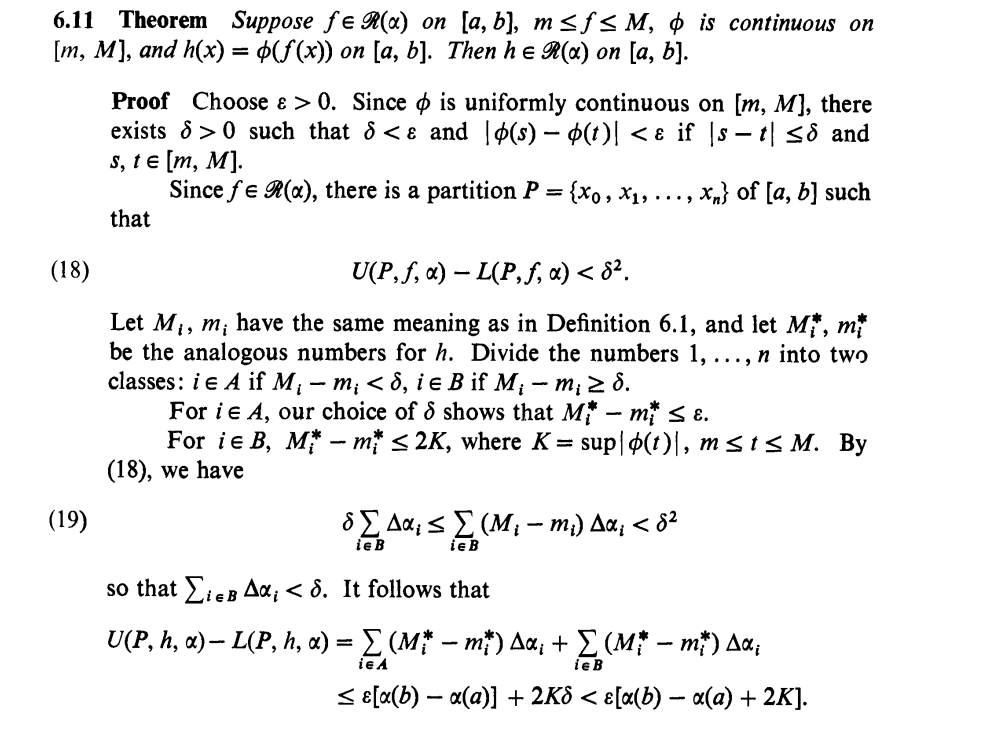
\includegraphics[scale=0.8]{theorem_6_11}

\subsection{Series of functions}

\subsection{Power series}

\paragraph{Radius of convergence}
Lemma. Let $\sum_n a_n(x-x_0)^n$ be convergent at $x_1$. Then $|x-x_0| < |x_1-x_0|$ implies $\sum_n a_n(x-x_0)^n$ converges absolutely.

\begin{itemize}
\item It is due to this lemma that we can speak of radius of convergence. Because of this lemma, radius of convergence as a concept can exist independently of the root test. 
\item However, the root test is a convenient way to find the radius of convergence since $\limsup$ is guaranteed to exist.
\item Additionally, the root test itself can be used to prove the above lemma.
\item Finally, we also note that the above lemma and the ratio test are related since both of their proofs make use of the geometric series.
\end{itemize}

\paragraph{Ratio test}
Given $\sum_n a_n$, consider $L_n = \lvert \frac{a_{n+1}}{a_n} \rvert$
\begin{itemize}
	\item if $\lim_{n\rightarrow \infty} L_n < 1$, converges
	\item if $\lim_{n\rightarrow \infty} L_n > 1$, diverges
	\item if $\lim_{n\rightarrow \infty} L_n = 1$, indeterminate
\end{itemize}

\subparagraph{Ratio test (variants)}
\begin{itemize}
	\item if $\limsup_{n\rightarrow \infty} L_n < 1$, converges
	\item if $\liminf_{n\rightarrow \infty} L_n > 1$, diverges
	\item if $L_n\geq 1$ for all but finitely many $n$, diverges
\end{itemize}

Note: If $L_n\geq 1$ for infinitely many $n$, the series can still converge.

\paragraph{Property of limsup}
Given that $(a_n)$ converges,
\begin{align*}
	\limsup_{n\rightarrow \infty} a_nb_n = \lim_{n\rightarrow \infty} a_n\cdot \limsup_{n\rightarrow \infty} b_n
\end{align*}

\paragraph{Uniform convergence of power series} Let $\sum_n a_n(x-x_0)^n$ have radius of convergence $R>0$. Then for any $[a,b]\subseteq (x_0-R, x_0+R)$, the series converges uniformly on $[a,b]$.

This property of power series means we get some extent of uniform convergence for free.

\paragraph{Differentiability of power series} Let $f(x)=\sum_{n=0}^\infty a_n(x-x_0)^n$ have radius of convergence $R>0$. Then $f\in C^{\infty}(x_0-R, x_0+R)$. And $\forall k\in \mathbb{Z}^+_0$
\begin{align*}
	f^{(k)}(x) = \sum_{n=k}^\infty n^{\underline{k}}(x-x_0)^{n-k}
\end{align*}
on $(x_0-R, x_0+R)$. In particular, the radius of convergence of $f^{(k)}$ is $R$, though the domain of convergence can be any of $[x_0-R, x_0+R], (x_0-R, x_0+R], [x_0-R, x_0+R), (x_0-R, x_0+R)$.

The proof is by taking the union over any $[x_0 - r, x_0 + r], r<R$ to give differentiability over the entire $(x_0-R, x_0+R)$.

Note: Properties like continuity and differentiability can be generalized by union.

\paragraph{Uniqueness of power series} Suppose a function $f$, there is a power series such that $f(x) = \sum_n a_n(x-x_0)^n$ on $(x_0-r, x_0+r)$. Here, $r$ must clearly be $\leq$ radius of convergence $R$. Then, $\forall k\in \mathbb{Z}^+_0$
\begin{align*}
	f^{(k)}(x_0) = k^{\underline{k}}a_k = k!a_k
\end{align*},
that is, \begin{align*}
	a_k = \frac{f^{(k)}(x_0)}{k!}
\end{align*}

Hence $\sum_n a_n(x-x_0)^n = \sum_n b_n(x-x_0)^n$ on some on $(x_0-r, x_0+r), r>0$ implies $\forall n, a_n = b_n$.

\paragraph{Summation by parts} Given sequences $(b_n, c_n)$. Let $B_{n,m}=\sum_{m\leq k\leq n}b_k$. Then,
\begin{align*}
	\sum_{m\leq k\leq n} b_kc_k = B_{n,m}c_n + \sum_{m\leq k\leq n-1}B_{k,m}(c_k - c_{k+1})
\end{align*}
This can be used to prove both Dirichlet's and Abel's test.

\paragraph{Corollary to Abel's Theorem} Suppose
\begin{align*}
	f(x) = \sum_n a_n(x-x_0)^n
\end{align*}
on $(x_0-R, x_0+R)$ and the power series converges at $x=x_0+R$.

Here, we can view $f$ as the closed form. Let $g$ represent the power series. Abel's theorem says that $g$ is defined on $(x_0-R, x_0+R]$ and the convergence to $g$ is uniform on $[x_0, x_0+R]$. In particular, $g$ is continuous at $x_0+R$. Hence, we have,
\begin{align*}
	g(x_0+R) = \lim_{x\rightarrow (x_0+R)^-}g(x) = \lim_{x\rightarrow (x_0+R)^-}f(x)
\end{align*}
If we extend $f$ to $(x_0-R, x_0+R]$ (assuming that the closed form $f$ is defined at $x_0+R$), and supposing $f$ is also continuous at $x_0+R$, then we have $g(x_0+R) = f(x_0+R)$. This allows us to equate
\begin{align*}
	f(x_0+R) = g(x_0+R) = \sum_n a_nR^n
\end{align*}

\paragraph{Merten's Theorem} Given $(a_n),(b_n)$, suppose $\sum_n a_n$ converges absolutely and $\sum_n b_n$ converges. Let $c_n = \sum_{0\leq k\leq n} a_k b_{n-k}$. Then,
\begin{align*}
	\sum_{n\geq 0}c_n = \sum_{n\geq 0}a_n\sum_{n\geq 0}b_n
\end{align*}

Corollary. We adjust the starting indices of $(a_n), (b_n)$. Suppose $\sum_{n\geq N_1}a_n$ converges absolutely and $\sum_{n\geq N_2}b_n$ converges. Then,
\begin{align*}
	\sum_{n\geq N_1 + N_2}\sum_{N_1\leq k\leq n-N_2}a_kb_{n-k} = \sum_{n\geq N_1}a_n\sum_{n\geq N_2}b_n
\end{align*}

The proof is by defining $a_k, k < N_1$ and $b_k, k < N_2$ to be $0$. Hence,
\begin{align*}
	\sum_{n\geq N_1}a_n\sum_{n\geq N_2}b_n = \sum_{n\geq 0}\sum_{0\leq k\leq n}a_kb_{n-k}a_kb_{n-k}[k\geq N_1][n-k\geq N_2]
\end{align*}
and observing that $[k\geq N_1][n-k\geq N_2] = [k\geq N_1][n-k\geq N_2][k+n-k\geq N_1+N_2] = [k\geq N_1][n-k\geq N_2][n\geq N_1+N_2]$.

Application. Consider a power series $\sum_n a_n(x-x_0)^n$ with radius of convergence $R$. Then if $x\in (x_0-R, x_0+R)$, $\sum_n a_n(x-x_0)^n$ converges absolutely. This allows us to apply Merten's theorem when concerning products of power series.

\paragraph{Analytic functions} A function $f$ is analytic on $(a,b)$ if
\begin{enumerate}
	\item $f\in C^\infty(a,b)$
	\item $\forall x_0\in (a,b)$, $f$ is equal to its Taylor series with basepoint at $x_0$ in some neighborhood of $x_0$.
\end{enumerate}

Lemma. If for a certain $x_0\in (a,b)$, $f$ equals to its Taylor series with basepoint at $x_0$ over $(a,b)$, then $f$ is analytic on $(a,b)$.

\subsection{Special functions}
\paragraph{Characterization of trig functions} If $g:\mathbb{R}\rightarrow \mathbb{R}$ has the property, $\forall x\in \mathbb{R}$
\begin{align*}
	g''(x) = -g(x)
\end{align*}, then $g(x) = g(0)\cos(x) + g'(0)\sin(x)$.

\paragraph{Characterization of exponential functions} If $E$ is a real function such that
\begin{align*}
	E'(x) = E(x) \land E(0) = 1
\end{align*}
on $\mathbb{R}$, then $E=\exp$.

\end{document}


